%! TeX program = lualatex
\documentclass[main]{subfiles}

\begin{document}

\providecommand{\Var}{\operatorname{Var}}  % \Var not in global macros

\title[AutoML: BO]{Bayesian Optimization}
\subtitle{Random Forest Surrogates}
\author[Bernd Bischl]{Bernd Bischl}
\date{}

\titlebackground*{images/AutoML_HPO_bayesian3.jpg}

    \maketitle


\begin{frame}[t]{Why Use a Random Forest as Surrogate?}
% \footnotesize
\begin{columns}[onlytextwidth,T]
  \column{.6\textwidth}
  \begin{itemize}
    \item GPs struggle 
        \begin{itemize}
            \item mixed / hierarchical $\pcs$ 
            \item high-dimensional or large $n$
        \end{itemize}
    \item Random forests handle all these naturally:
        \begin{itemize}
            \item Tree splits work on categorical and conditional features without a kernel
            \item Training complexity $\mathcal{O}(B \cdot n \log n)$;\\
            B is ensemble size
            \item Robust
        \end{itemize}
    \item Downside: RFs not Bayesian\\
    $\leadsto$ uncertainty estim. less clear
    \item SMAC~\liturl{Hutter et al. 2011}{https://link.springer.com/chapter/10.1007/978-3-642-25566-3_40} classical example, uses BO with RF
  \end{itemize}
  \column{.4\textwidth}
  \begin{center}
    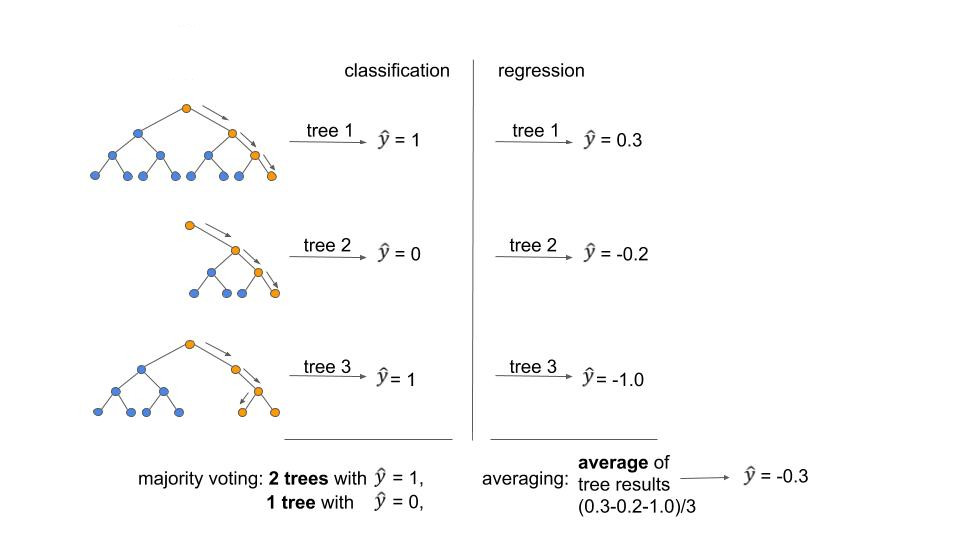
\includegraphics[width=\textwidth]{images/random_forests.jpg}
  \end{center}
\end{columns}
\end{frame}


% \begin{frame}[t]{Sources of Randomness in a Random Forest}
%   To build an RF we inject randomness at three stages:
%   \begin{itemize}
%     \item \textbf{Bagging:} each tree $b$ trained on a bootstrap sample of $\hist$
%     \item \textbf{Feature subsampling:} at each split, only $m \le \pcsdim$ features are considered
%     \item \textbf{Random split locations} (\textbf{extratrees}): cut point chosen uniformly at random inside the feature's range
%   \end{itemize}
%   \vspace{0.2cm}
%   \textbf{Key idea for BO:} the spread of per-tree predictions across the ensemble reflects \textbf{epistemic uncertainty} at $x$ -- high spread where data is scarce or the target is harder to model.
% \end{frame}


\begin{frame}[t]{Naive Variance from Per-Tree Predictions}
\begin{columns}[onlytextwidth,T]
  \column{.6\textwidth}
  \begin{itemize}
    \item Treat $B$ tree predictions $\hat{f}_b(x)$ as samples and take their empirical variance~\liturl{Hutter et al. 2014}{https://doi.org/10.1016/j.artint.2013.10.003}
    \item Forest mean: $\hat{f}(x) = \frac{1}{B} \sum_{b=1}^B \hat{f}_b(x)$
    \item Naive variance:
      $$
      \sh^2_{\text{naive}}(x) = \frac{1}{B-1} \sum_{b=1}^B \big(\hat{f}_b(x) - \hat{f}(x)\big)^2
      $$
    \item Captures only \textbf{between-tree disagreement};
    ignores spread of training labels within each leaf
  \end{itemize}
  \column{.4\textwidth}
  \begin{center}
    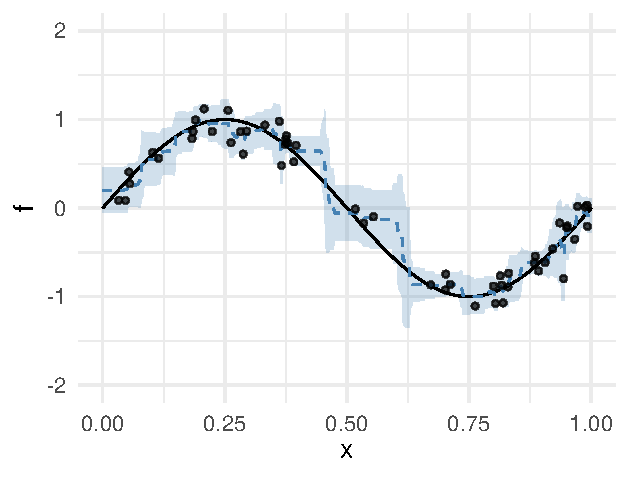
\includegraphics[width=\textwidth]{images/04_rf_unc_var_estimators_naive.pdf}\\
    {\scriptsize $\pm 2\sh_{\text{naive}}$ band; truth (black), forest mean (dashed)}
  \end{center}
\end{columns}
\end{frame}


\begin{frame}[t]{Mean and Variance via Law of Total Variance}
  \begin{itemize}
    \item Fix test point $x$ -- from here on everything is conditional on $x$ 
    \item Let $\hat{f}_b(x)$, $\sh_b^2(x)$ be mean and within-leaf variance of tree $b$
    \item Two-stage draw: $b \sim \text{Unif}\{1,\ldots,B\}$, then $Y \sim$ leaf distribution of tree $b$ at $x$
    \item Conditionals: $\E[Y \mid b] = \hat{f}_b(x)$, $\Var(Y \mid b) = \sh_b^2(x)$
    \item Law of total variance: $\Var(Y) = \E_b[\Var(Y \mid b)] + \Var_b(\E[Y \mid b])$ becomes
    $$
    \sh^2(x) = \underbrace{\frac{1}{B} \sum_{b=1}^B \sh_b^2(x)}_{\text{within-tree (aleatoric)}}
      + \underbrace{\frac{1}{B} \sum_{b=1}^B \hat{f}_b(x)^2 - \hat{f}(x)^2}_{\text{between-tree (epistemic)}}
    $$
    \item Also from \liturl{Hutter et al. 2014}{https://doi.org/10.1016/j.artint.2013.10.003}, used in SMAC and most RF-based BO implementations
  \end{itemize}
\end{frame}


\begin{frame}[t]{Jackknife-Based Variance Estimators}
  \begin{itemize}
    \item \textbf{Infinitesimal jackknife (IJ)}~\liturl{Wager et al. 2014}{https://jmlr.org/papers/v15/wager14a.html} gives a formally grounded variance estimate:
        $$\widehat{\sh}^2_{IJ}(x) = \sum_{i=1}^n \Big(\operatorname{Cov}_b(N_{ib}, \hat{f}_b(x))\Big)^2$$
        where $N_{ib}$ is how often observation $i$ appears in bootstrap sample $b$
    \item Bias-corrected variant removes systematic bias in finite forests
    \item Captures uncertainty that the law-of-total-variance estimator misses\\
    (esp.\ for small $B$)
    \item More expensive than the basic mean-of-variances, but tractable
  \end{itemize}
\end{frame}


\begin{frame}[t]{Extra-Trees: Random Split Locations}
\begin{columns}[onlytextwidth,T]
  \column{.6\textwidth}
  \begin{itemize}
    \item Standard RF: at each node, pick \textbf{empirically best} split (max L2 loss reduction)
    \item \textbf{Extra-trees}~\liturl{Geurts et al. 2006}{https://link.springer.com/article/10.1007/s10994-006-6226-1}: pick the split point \textbf{uniformly at random} per candidate feature
    \item Trade-offs:
        \begin{itemize}
            \item Faster training -- no scan over candidate splits
            \item More between-tree disagreement $\leadsto$ smoother $\hat f$
            \item Slightly higher bias per tree, lower variance after averaging
        \end{itemize}
  \end{itemize}
  \column{.4\textwidth}
  \begin{center}
    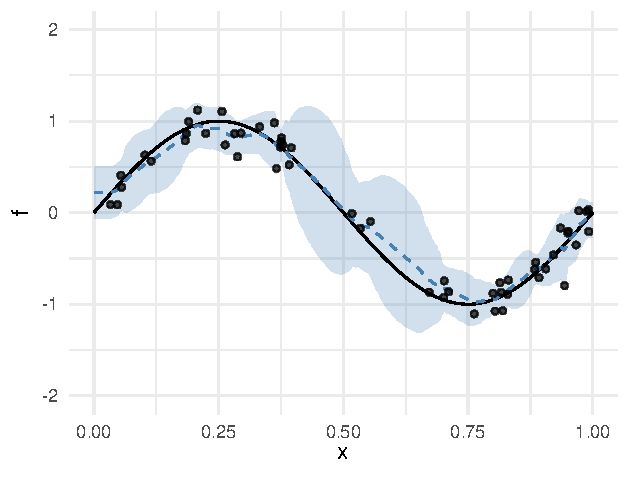
\includegraphics[width=\textwidth]{images/04_extra_trees.pdf}\\
    {\scriptsize $\pm 2\sh$ band from per-tree disagreement; mean (dashed)}
  \end{center}
\end{columns}
\end{frame}


\begin{frame}[t]{Quantile Regression Forests}
\footnotesize
\begin{columns}[onlytextwidth,T]
  \column{.6\textwidth}
  \begin{itemize}
    \item \textbf{Quantile regression forests}~\liturl{Meinshausen 2006}{https://jmlr.org/papers/v7/meinshausen06a.html}: keep the entire \textbf{empirical leaf distribution} of training labels, not just per-leaf means
    \item Aggregate per-tree leaf labels (weighted) to approximate $F(y \mid x)$
    \item From this CDF:
        \begin{itemize}
            \item predictive \textbf{quantiles} 
            \item predictive \textbf{mean} and \textbf{variance}
            \item \textbf{non-Gaussian} predictive distributions
        \end{itemize}
    \item Natural fit with AFs that need quantiles or samples (LCB, Thompson sampling)
  \end{itemize}
  \column{.4\textwidth}
  \begin{center}
    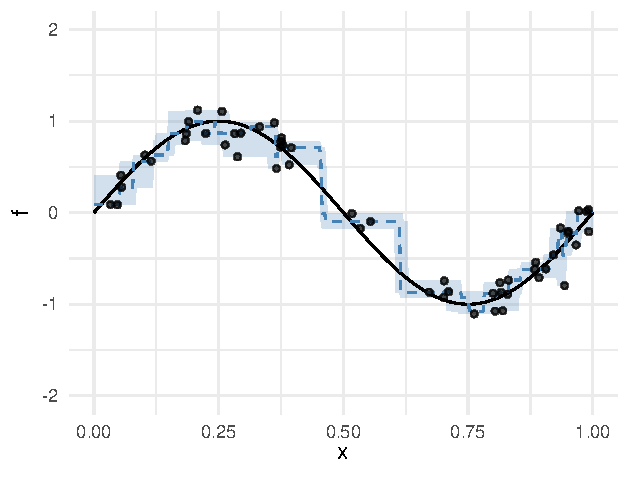
\includegraphics[width=\textwidth]{images/04_rf_unc_var_estimators_qrf.pdf}\\
    {\scriptsize 10/50/90\% quantile band; truth (black), median (dashed)}
  \end{center}
\end{columns}
\end{frame}


% \begin{frame}[t]{Smoothing Tricks}
%   RF predictions are piecewise constant $\leadsto$ acquisition-function landscape is also piecewise constant:
%   \begin{itemize}
%     \item Kills gradient-based AF optimization
%     \item Can make exploration criteria plateau / tie in many points
%   \end{itemize}
%   \vspace{0.2cm}
%   Common workarounds:
%   \begin{itemize}
%     \item \textbf{Extra-trees}: random split locations $\leadsto$ ``smoother'' mean
%     \item \textbf{Kernel smoothing}: replace per-leaf mean with a locally-weighted average
%     \item \textbf{Increase $B$}: more trees average out step-wise structure
%     \item \textbf{Use a different AF optimizer}: random search / EA, since gradients don't help anyway
%   \end{itemize}
% \end{frame}


\begin{frame}[t]{Summary and Discussion}
\begin{itemize}
  \item Use RF for mixed / conditional / large-integer $\pcs$, large $n$, cheaper $f$ with many iterations;
  GP for numeric $\pcs$ with tighter budget
  \item We discussed as uncertainty options:\\
  naive between-tree variance, law of total variance, infinitesimal jackknife, and quantile regression forests
  \item Extra-trees for further smoothing
  \item RF variance is not truly Bayesian; tends to \textbf{underestimate} in extrapolation zones, \textbf{overestimate} near the training data
  \item Works well in practice; rescale via held-out residuals if calibration matters
\end{itemize}
\end{frame}


\end{document}
